\documentclass{article}

\usepackage{GOST}
\usepackage[T1, T2A]{fontenc}
\usepackage[utf8]{inputenc}
\usepackage[russian]{babel}
\usepackage{cmap}
\usepackage{amssymb}
\usepackage{amsmath}
\usepackage{hyperref}

\usepackage{listings}
% Для листинга кода:
\lstset{ 
	language=C,                 % выбор языка для подсветки (здесь это С)
	basicstyle=\small\sffamily, % размер и начертание шрифта для подсветки кода
	numbers=left,               % где поставить нумерацию строк (слева\справа)
	numberstyle=\tiny,           % размер шрифта для номеров строк
	stepnumber=1,                   % размер шага между двумя номерами строк
	numbersep=5pt,                % как далеко отстоят номера строк от подсвечиваемого кода
	showspaces=false,            % показывать или нет пробелы специальными отступами
	showstringspaces=false,      % показывать или нет пробелы в строках
	showtabs=false,             % показывать или нет табуляцию в строках
	frame=single,              % рисовать рамку вокруг кода
	tabsize=2,                 % размер табуляции по умолчанию равен 2 пробелам
	captionpos=t,              % позиция заголовка вверху [t] или внизу [b] 
	breaklines=true,           % автоматически переносить строки (да\нет)
	breakatwhitespace=false, % переносить строки только если есть пробел
}


\graphicspath{{images/}}

\linespread{1.5}

\title{Отчет по анализу алгоритмов}
\date{2020}

\begin{document}
	\begin{table}[ht]
	\centering
	\begin{tabular}{|c|p{400pt}|} 
	\hline
		\begin{tabular}[c]{@{}c@{}} 
\includegraphics[scale=0.37]{EmblemBMSTU} \\\end{tabular} &
		\footnotesize\begin{tabular}[c]{@{}c@{}}\textbf{Министерство~науки~и~высшего~образования~Российской~Федерации}\\\textbf{Федеральное~государственное~бюджетное~образовательное~учреждение}\\\textbf{~высшего~образования}\\\textbf{«Московский~государственный~технический~университет}\\\textbf{имени~Н.Э.~Баумана}\\\textbf{(национальный~исследовательский~университет)»}\\\textbf{(МГТУ~им.~Н.Э.~Баумана)}\\\end{tabular}  \\
	\hline
	\end{tabular}
\end{table}
\noindent\rule{\textwidth}{4pt}
\noindent\rule[14pt]{\textwidth}{1pt}
\hfill 
\noindent
\makebox{ФАКУЛЬТЕТ~}%
\makebox[\textwidth][l]{\underline{~~~~«Информатика и системы управления»~~~~~~~~~~~~~~~~~~~~~~~~~~~~~~~~~~~~~~~~~~~~}}%
\\
\noindent
\makebox{КАФЕДРА~}%
\makebox[\textwidth][l]{\underline{~~~~~~~«Программное обеспечение ЭВМ и информационные технологии»~~~~~~~~}}%
\\


\begin{center}
	\vspace{3cm}
	{\bf\huge Отчёт\par}
	{\bf\Large по лабораторной работе № 2\par}
	\vspace{0.5cm}
\end{center}


\noindent
\makebox{\large{\bf Название:}~~~}
\makebox[\textwidth][l]{\large\underline{~Алгоритмы умножения матриц~~~~~~~~~~~~~}}\\

\noindent
\makebox{\large{\bf Дисциплина:}~~~}
\makebox[\textwidth][l]{\large\underline{~Анализ алгоритмов~~~~~~~~~~~~~~~~~~~~~~~~~~~~~~~~~~~~~~~~~~~~~~~~~~~~}}\\

\vspace{1.5cm}
\noindent
\begin{tabular}{l c c c c c}
    Студент      & ~ИУ7-55Б~               & \hspace{3.5cm} & \hspace{3.5cm}                 & &  Д.Р.Жигалкин \\\cline{2-2}\cline{4-4} \cline{6-6} 
    \hspace{3cm} & {\footnotesize(Группа)} &                & {\footnotesize(Подпись, дата)} & & {\footnotesize(И.О. Фамилия)}
\end{tabular}

\vspace{1cm}

\noindent
\begin{tabular}{l c c c c}
    Преподователь & \hspace{6cm}   & \hspace{3.5cm}                 & & Л.Л. Волкова \\\cline{3-3} \cline{5-5} 
    \hspace{3cm}  &                & {\footnotesize(Подпись, дата)} & & {\footnotesize(И.О. Фамилия)}
\end{tabular}

\begin{center}	
	\vfill
	\large \textit {Москва, 2020}
\end{center}

\thispagestyle {empty}
\pagebreak
	\newpage
	\tableofcontents
	\newpage
	\begin{center}
	    \section*{Введение}
	\end{center}
	\addcontentsline{toc}{section}{Введение}
    		Словарь -- книга или любой другой источник,
    информация в котором упорядочена c помощью разбивки на небольшие статьи,
    отсортированные по названию или тематике. 
    Различают энциклопедические и лингвистические словари.
    С развитием компьютерной техники всё большее распространение получают электронные словари и онлайн-словари.
    Первым русским словарём принято считать Азбуковник,
    помещённый в списке Кормчей книги 1282 года и содержащий 174 слова.
    Задача состоит в поиске слов из словаря в случайных данных любого размера(напр. в файле).
    Поскольку словарь меняется редко, то можно его подготовить
    (напр. отсортировать, создать дерево итд). 
    Это зависит от алгоритма поиска, который будет использован. 

    Целью данной лабораторной работы является реализация 
    алгоритмов поиска слов в словаре и исследование их трудоемкости.


    Задачи данной лабораторной работы:
    \begin{enumerate}
        \item описать алгоритм полного перебора;
        \item описать алгоритм двоичного поиска;
        \item описать алгоритм поиска слов по сегментам;
        \item реализовать 3 алгоритма поиска по словарю;
        \item провести замеры времени работы алгоритмов.
    \end{enumerate}
	\newpage
	\section{Аналитическая часть}
	В данном разделе будут поставлены цели и задачи работы, будут рассмотренны основные теоритические сведения связанные с алгоритмами сортировки.
		\subsection{Цель и задачи работы}
    Целью данной лабораторной работы является реализация 
    алгоритмов поиска слов в словаре и исследование их трудоемкости.

    Задачи данной лабораторной работы:
    \begin{enumerate}
        \item описать алгоритм полного перебора;
        \item описать алгоритм двоичного поиска;
        \item описать алгоритм поиска слов по сегментам;
        \item реализовать 3 алгоритма поиска по словарю;
        \item провести замеры времени работы алгоритмов.
    \end{enumerate}

		\subsection{Алгоритм полного перебора}
		Алгоритм полного перебора подразумевает проверку каждого элемента множества.  В случае словаря проверяется каждый элемент словаря на соответствие ключу.
Сложность - n.
		\subsection{Алгоритм двоичного поиска}
		Алгоритм двоичного поиска осуществляет поиск по упорядоченному множеству объектов. \newline
		\indent Двоичный поиск заключается в том, что на каждом шаге множество объектов делится на две части и в работе остаётся та часть множества, где находится искомый объект. Или же, в зависимости от постановки задачи, мы можем остановить процесс, когда мы получим первый или же последний индекс вхождения элемента. Последнее условие — это левосторонний/правосторонний двоичный поиск \cite{binary-search}.
		\subsection{Алгоритм поиска по сегментам}
		\indent Для применения этого алгоритма множество разбивается на сегменты по определеннуму признаку. При поиске у ключевого элемента определяется сначала этот признак, а затем осуществляется поиск по соответствующему сегменту множества.
	\subsection{Вывод}
	В данной части были поставлены задачи и цель работы, описаны алгоритмы полного перебора, двоичного поиска, поиска по сегментам.
	\newpage
	\section{Конструкторская часть}
		В данном разделе будут рассмотренны схемы алгоритмов, требования к функциональности ПО.
		\subsection{Требования к ПО} 
		ПО должно иметь два режима работы, выбираемые из меню:
		\begin{enumerate}
			\item режим демонстрации. В этом режиме должен осуществляться ввод слова и последующий поиск его в словаре с помощью всех алгоритмов;
		 	\item режим тестирования. В этом режиме должны проводится замеры времени выполнения реализованных алгоритмов.
	 	\end{enumerate}
		\subsection{Схемы алгоритмов}
		На \hyperref[bruteForceAlg]{рисунке \ref{bruteForceAlg}} изображена схема алгоритма полного перебора.
	\begin{figure}[h!]
		\center{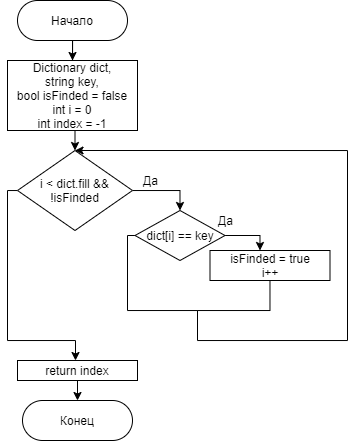
\includegraphics{bruteForceAlg.png}}
		\caption{Схема алгоритма полного перебора}
		\label{bruteForceAlg}
	\end{figure}
	\newpage

		На \hyperref[binarySearchAlg]{рисунке \ref{binarySearchAlg}} изображена схема алгоритма двоичного поиска.
	\begin{figure}[h!]
		\center{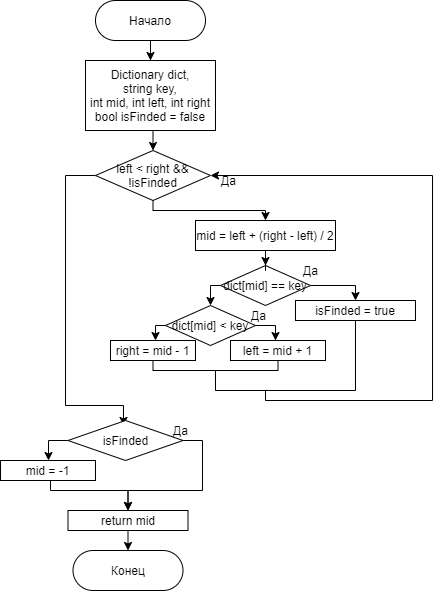
\includegraphics{binarySearchAlg.png}}
		\caption{Схема алгоритма двоичного поиска}
		\label{binarySearchAlg}
	\end{figure}
	\newpage

На \hyperref[segmentAlg]{рисунке \ref{segmentAlg}} изображена схема алгоритма поиска по сегментам.
	\begin{figure}[h!]
		\center{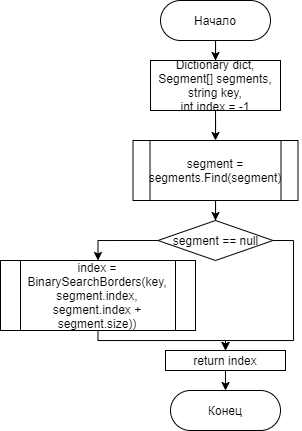
\includegraphics{segmentAlg.png}}
		\caption{Схема алгоритма поиска по сегментам}
		\label{segmentAlg}
	\end{figure}
	\newpage

	\subsection{Вывод}
	В данном разделе были рассмотрена реализуемое ПО и обозначены требования к нему.
	
	\newpage
	\section{Технологическая часть}
	Ниже будут представлены средства реализации и листинги реализованной программы.
	\subsection{Средcтва реализации}
	Выбранный язык программирования - C\#, так как имеется практический опыт разработки на нём \cite{c-sharp}. Среда разработки - Visual Studio \cite{vs}.
\newline
	\indent Технические характеристики машины, на которой проводились тесты:
	\begin{itemize}
	\item Windows 10 x64;
	\item 8 ГБ оперативной памяти;
	\item CPU: AMD FX(tm)-8300 Processor 4.5GHz;
	\item 8 логических ядер.
	\end{itemize}	
	\subsection{Реализации алгоритмов}
	Ниже представлены листинг класса Dictionary, реализующего весь функционал. Метод BruteForce реализует полный перебор, BinarySearch - бинарный поиск, FindBySegments - поиск по сегментам.


		На листинге \hyperref[dictLst]{\ref{dictLst}} представлен класс Dictionary.
	\begin{lstlisting}[label=dictLst,caption=Dictionary]
    class Dictionary
    {
        string[] body;
        Segment[] segments;
        int segmentsCount = 0;
        public int fill = 0;
        public string this[int i]
        {
            get { return body[i]; }
            set { body[i] = value; }
        }   

        public Dictionary(string pathToFile)
        {
            if (File.Exists(pathToFile))
            {
                body = new string[100];
                using (StreamReader sr = File.OpenText(pathToFile))
                {
                    string s;
                    fill = 0;
                    while ((s = sr.ReadLine()) != null)
                    {
                        if (fill == body.Length)
                        {
                            Array.Resize(ref body, (int)(fill * 1.5));
                        }
                        this[fill] = s.ToLower();
                        fill++;
                    }
                }
                Array.Resize(ref body, fill);
                Sort();
                FormSegments();
            }
        }

        public void Sort()
        {
            Array.Sort(body);
        }

        public void FormSegments()
        {
            if (fill > 0)
            {
                segments = new Segment[33];
                segmentsCount = 0;
                char key = this[0][0];
                int indexStart = 0;
                for (int i = 1; i < fill; i++)
                {
                    if (key != this[i][0])
                    {
                        if (segmentsCount == segments.Length)
                        {
                            Array.Resize(ref segments, (int)(segmentsCount * 1.5));
                        }
                        segments[segmentsCount] = (new Segment(key, indexStart, i - indexStart));
                        segmentsCount++;
                        key = this[i][0];
                        indexStart = i;
                    }
                }
                segments[segmentsCount] = (new Segment(key, indexStart, fill - indexStart));
                segmentsCount++;
                Array.Resize(ref segments, segmentsCount);
                Array.Sort(segments);
            }
        }
        // return index of key
        public int BruteForce(string key)
        {
            int index = -1;
            bool isFinded = false;
            for (int i = 0; i < fill && !isFinded; i++)
            {
                if (key.CompareTo(this[i]) == 0)
                {
                    isFinded = true;
                    index = i;
                }
            }

            return index;
        }

        public int BinarySearch(string key)
        {
            return BinarySearchBorders(key, 0, fill);
        }

        private int BinarySearchBorders(string key, int left, int right)
        {
            int mid = 0;
            int finded = 1;
            bool isFinded = false;

            while (!isFinded && left < right)
            {
                mid = left + (right - left) / 2;
                finded = key.CompareTo(this[mid]);
                if (finded == 0)
                {
                    isFinded = true;
                }
                else if (finded < 0)
                {
                    right = mid - 1;
                }
                else
                {
                    left = mid + 1;
                }
            }
            mid = isFinded ? mid : -1;
            return mid;
        }

        public int FindBySegments(string key)
        {
            int index = -1;
            char keyChar = key[0];
            Segment segment = Array.Find(segments, (a) => (a.key == keyChar));

            if (segment != null)
                index = BinarySearchBorders(key, segment.index, segment.index + segment.size);
            return index;
        }
    }
	\end{lstlisting}

	\subsection{Вывод}
	В данном разделе были описаны программные и аппаратные средства реализации, были представлены листинги программы.

	\newpage
	\section{Экспериментальная часть}
	В данной главе будет представлен пример работы программы и представлены результаты замера времени поиска.
	\subsection{Пример работы программы}
	Пример работы программы представлен на рисунке \hyperref[programmWork]{\ref{programmWork}}
	 	\begin{figure}[h!]
		 	\center{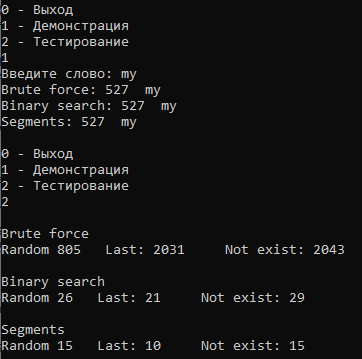
\includegraphics[scale=0.9]{programmWork.png}}
		 	\caption{Пример работы программы}
		 	\label{programmWork}
	 	\end{figure}

	\subsection{Тесты}
	Тесты проводятся на словаре из 1000 элементов с шагом 25. По оси абсцисс отложено место искомого слова в словаре. Результаты тестирования представлены на рисунке \hyperref[tests]{\ref{tests}}
	 	\begin{figure}[h!]
		 	\center{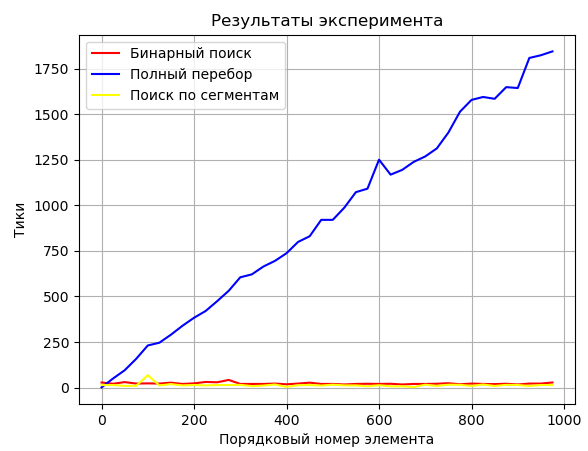
\includegraphics[scale=0.9]{tests.png}}
		 	\caption{Результаты эксперимента}
		 	\label{tests}
	 	\end{figure}
	\newpage

	\subsection{Вывод}
	Из проведенного эксперимента можно сделать вывод, что алгоритм полного перебора самый медленный из реализованных алгоритмов, а алгоритм поиска по сегментам - самый быстрый. Это свзяано с тем, что при поиске по сегментам необходимо заранее отсекать большую часть проверяемых слов.

	\newpage
	\begin{center}
		\section*{Заключение}
	\end{center}
	\addcontentsline{toc}{section}{Заключение}
	\indent \indent В ходе выполнения данной лабораторной работы была достигнута её цель -  реализация 
    алгоритмов поиска слов в словаре и исследование их трудоемкости. 

Для этого были выполнены следующие задачи:

    \begin{enumerate}
        \item описан алгоритм полного перебора;
        \item описан алгоритм двоичного поиска;
        \item описан алгоритм поиска слов по сегментам;
        \item проведен замер времени работы алгоритмов.
    \end{enumerate}

	Из проведенного эксперимента был сделан вывод, что алгоритм полного перебора самый медленный из реализованных алгоритмов, а алгоритм поиска по сегментам - самый быстрый. Это свзяано с тем, что при поиске по сегментам необходимо заранее отсекать большую часть проверяемых слов.

	\newpage
	\addcontentsline{toc}{section}{Список литературы}
	
	\begin{center}
	\begin{thebibliography}{3}
	\bibitem{binary-search}
	Целочисленный двоичный поиск. ITMO [Электронный ресурс]. Режим доступа: (дата обращения - 20.11.2020) Свободный. URL: https://neerc.ifmo.ru/wiki/index.php?title=Целочисленный\_двоичный\_поиск
	\bibitem{c-sharp}
	C\# [Электронный ресурс]. Режим доступа: (дата обращения - 20.11.2020) Свободный. URL: https://ru.wikipedia.org/wiki/C\_Sharp
	\bibitem{vs}
	Visual Studio [Электронный ресурс]. Режим доступа: (дата обращения - 20.11.2020) Свободный. URL: https://visualstudio.microsoft.com/ru/

	\end{thebibliography}
	\end{center}
\end{document}